\documentclass[10pt,twocolumn,letterpaper]{article}

% CVPR/ICCV submission template (draft-standalone preamble).
% Swap for \usepackage[review]{cvpr} + the official cvpr.sty when packaging.
\usepackage[margin=0.9in]{geometry}
% \usepackage{times}  % enable with official template (needs courier TFM)
\usepackage{graphicx}
\usepackage{amsmath,amssymb}
\usepackage{booktabs}
\usepackage{multirow}
\usepackage{xcolor}
\usepackage[colorlinks=true,allcolors=blue]{hyperref}
\usepackage{caption}
\usepackage{float}

\graphicspath{{figs/}}
\renewcommand{\ttdefault}{cmtt}

\title{Selective Disocclusion Prior Distillation for\\ Feed-Forward Single-View 3D Reconstruction}
\author{Anonymous submission\\\small Paper ID ****}
\date{}

\begin{document}
\maketitle

\begin{abstract}
A generative teacher can improve disoccluded regions, but it is expensive and
non-monotonic: on some scenes it is worse than the feed-forward baseline. We
study whether its useful behavior can be distilled within a high-teacher-gain
regime. We curate training and evaluation scenes using teacher-minus-baseline
invisible-region quality measured against ground truth, train an image-space
student, and copy baseline pixels in visible regions using masks derived offline
from the full target clip. This oracle curation and oracle visibility constitute
an upper-bound experiment, not deployable single-view inference. On a
4-scene/161-frame selected holdout, the student improves invisible-region PSNR
by \textbf{$+5.77$ dB} (teacher: $+6.09$ dB; 0.32 dB gap; 94.7\% retained)
with exactly zero visible change, while running in \textbf{0.087 s/scene versus
247 s}, a \textbf{$2833\times$ speedup}. A fixed custom 759-frame diagnostic
shows that the student improves LPIPS and FID over the feed-forward evidence
component while trailing the teacher on both metrics; it is not an official
Flash3D-protocol comparison. A negative ablation shows that recoloring
source-plane Gaussians with frozen geometry lacks support at newly disoccluded
target pixels. Deployment would require both selection and visibility estimated
only from inference-time observables; neither is established here.
\end{abstract}

\section{Introduction}
\label{sec:intro}
A generative reconstruction teacher guided by feed-forward geometry evidence
such as Flash3D~\cite{flash3d} can improve disoccluded regions, but requires a
slow diffusion denoise. More importantly, the teacher is non-monotonic: it helps
hard disocclusions and can hurt easy scenes. The central question is therefore
whether useful teacher behavior can be compressed under a clearly delimited
high-gain condition.

A naive residual network trained on every teacher render copies both successful
and harmful behavior. We instead study \emph{selective disocclusion prior
distillation}: scenes are selected using teacher and ground-truth outcomes, and
the student is trained and evaluated within that selected regime. This selection
is oracle dataset curation. It does not establish a mechanism for deciding on an
unseen scene whether the student should be used.

\paragraph{Contributions.}
\begin{enumerate}
\item \textbf{Conditional principle:} distillation of a non-monotonic teacher on
an oracle-curated high-teacher-gain regime, explicitly presented as an upper
bound rather than an inference-time selection result.
\item \textbf{Model and evidence:} a 46,371-parameter image-space student that
achieves $+5.77$ dB held-out invisible-region gain (teacher: $+6.09$ dB), exact
visible identity, and a $2833\times$ speedup; a fixed custom 759-frame diagnostic
reports the quality--speed tradeoff without claiming an official-protocol win.
\item \textbf{Architectural diagnosis:} a color-only Gaussian adapter recovers
only $\sim$7\% of the gap when overfit and gives $-1.72$ dB on holdout; a support
schematic explains why this motivates image-space correction.
\end{enumerate}

\section{Method}
\label{sec:method}

\begin{figure*}[t]
\centering
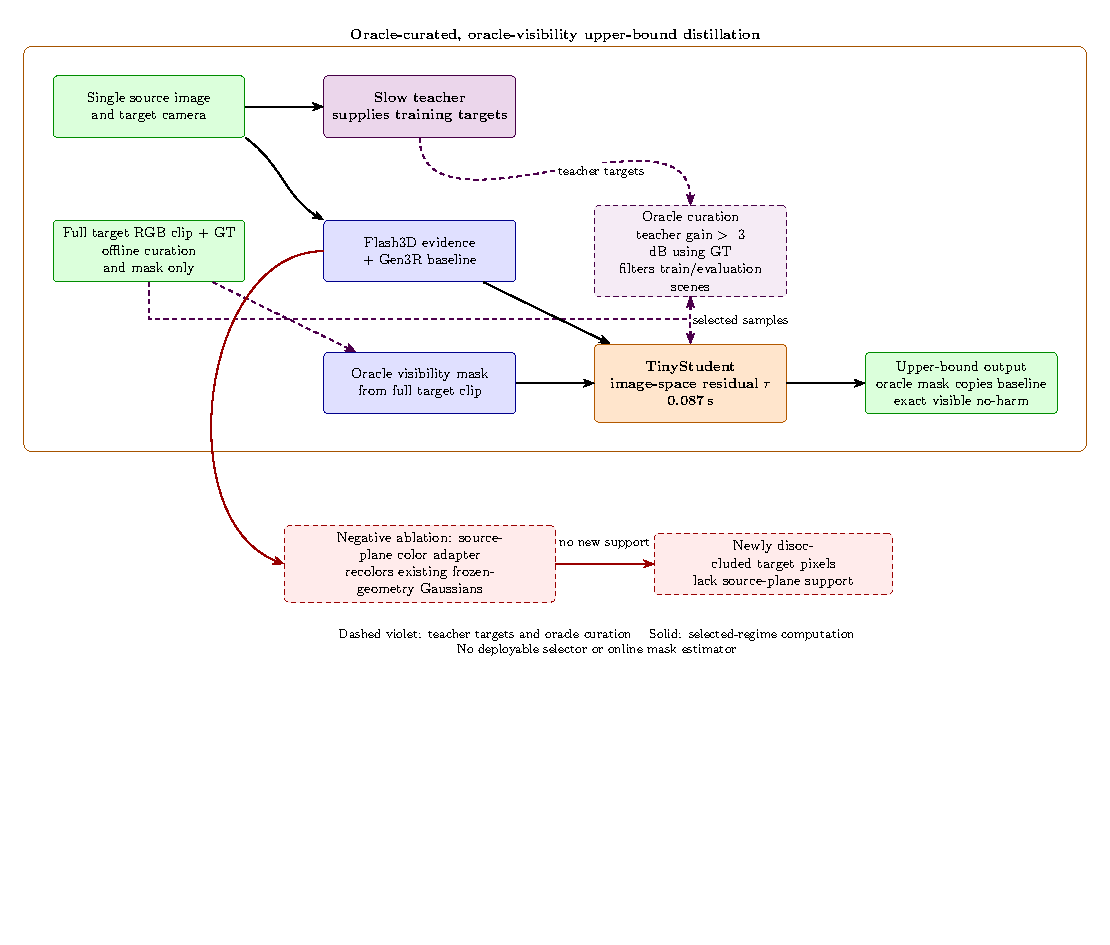
\includegraphics[width=0.9\textwidth]{fig_pipeline.pdf}
\caption{Oracle-selected distillation of a non-monotonic teacher. Teacher and
ground-truth outcomes select high-gain scenes for training and evaluation, while
the full target clip supplies oracle visibility. Within this selected regime, the
46,371-parameter CNN predicts an image-space residual from geometry evidence, the
baseline, and visibility; the visible mask copies baseline pixels exactly. There
is no inference-time selection or online mask-estimation mechanism in the reported
pipeline. The lower schematic summarizes the E-150 negative ablation:
a source-plane color adapter can recolor existing frozen-geometry Gaussians but
cannot create support for newly disoccluded target pixels. It is an explanation
of the measured ablation, not an invented render comparison.}
\label{fig:pipeline}
\end{figure*}

\subsection{Teacher and oracle scene selection}
The teacher is the slow selective-injection method: a generative backbone refined
by geometry-expert-guided disocclusion injection. It provides high-quality
disocclusion targets on hard scenes but is not universally better than the
baseline. We compute teacher-minus-baseline invisible-region PSNR against ground
truth and retain scenes whose gain exceeds 3 dB. Because this criterion uses the
teacher output and ground truth, it is oracle dataset curation and defines an
upper-bound condition for training and evaluation.

\subsection{Image-space student}
The student operates on rendered frames. Its input is
\texttt{[f3d\_rgb, baseline\_rgb, visibility\_mask, invisible\_mask]}; a small
convolutional network predicts a residual $r$ and outputs
\[
\text{student} = M\odot\text{baseline} + (1-M)\odot(\text{f3d}+r),
\]
so visible pixels ($M{=}1$) are copied from the baseline. Training uses
invisible-region L1 losses to teacher and GT plus a visible-region identity loss.
The visible mask therefore enforces exact no-harm inside each evaluated output;
it does not decide whether a scene belongs to the selected regime. These masks
are computed offline from the full target clip and are oracle information, not a
single-view model prediction.

\subsection{Scope of selection}
For evaluation on the reported selected holdout, the student is applied directly
with the precomputed oracle visibility mask. No learned or rule-based observable
selector or online mask estimator is validated here. General use on unseen,
uncurated scenes would require both components to use inputs available without
teacher renders, target clips, or ground truth.

\section{Experiments}
\label{sec:exp}
All PSNR numbers are \textbf{invisible-region} (disocclusion) PSNR, the targeted
quantity; visible-region PSNR is a no-harm check.

\subsection{Distillation on selected scenes}
We train the image-space student on scenes where the teacher beats the baseline
by more than 3 dB in invisible-region PSNR, using full per-frame teacher renders,
with a 4-scene / 161-frame held-out split drawn from the same oracle-selected
regime.

\begin{table}[t]
\centering\small
\caption{Distillation results (invisible-region PSNR) conditional on oracle
high-teacher-gain selection. The feed-forward student retains 94.7\% of the
teacher's held-out gain and leaves visible regions exactly unchanged.}
\resizebox{\columnwidth}{!}{%
\begin{tabular}{lrrrrr}
\toprule
Split & Base & Teacher & Student & Stud$-$Base & Vis $\Delta$ \\
\midrule
Train (n=696) & 15.31 & 20.68 & 20.80 & $\mathbf{+5.49}$ & $+0.000$ \\
Holdout (n=161) & 14.04 & 20.13 & 19.81 & $\mathbf{+5.77}$ & $+0.000$ \\
\bottomrule
\end{tabular}%
}
\end{table}
The student retains $5.77/6.09=94.7\%$ (approximately 95\%) of the teacher's
held-out gain and trails its PSNR by 0.32 dB (19.81 versus 20.13 dB), with visible
regions exactly unchanged. The gain is stable across held-out splits ($+5.96$
and $+4.75$ dB during scaling).

\subsection{Scope of the reported regime}
On scenes where the teacher does not outperform the baseline, the student is
flat-to-slightly-negative because there is no useful teacher signal to copy.
This observation motivates oracle high-gain curation but does not solve selection
from observable inputs. Results in this paper must therefore be interpreted as
conditional performance on the curated regime.

\subsection{Runtime}
\begin{table}[H]
\centering\small
\caption{Runtime and quality on the selected regime. The student is four
$3\times3$ convolutions applied once per frame; the teacher requires a 30-step
diffusion denoise of the clip.}
\resizebox{\columnwidth}{!}{%
\begin{tabular}{lrrr}
\toprule
Method & Time/scene & Inv $\Delta$ & Visible \\
\midrule
Teacher (30-step diffusion) & 247 s & $+6.09$ & lossless \\
\textbf{Fast student (CNN)} & \textbf{0.087 s} & $\mathbf{+5.77}$ & lossless \\
Speedup & $\mathbf{2833\times}$ & 94.7\% kept ($\sim$95\%) & --- \\
\bottomrule
\end{tabular}%
}
\end{table}

\subsection{Fixed custom 759-frame quality--speed diagnostic}
\begin{figure}[H]
\centering
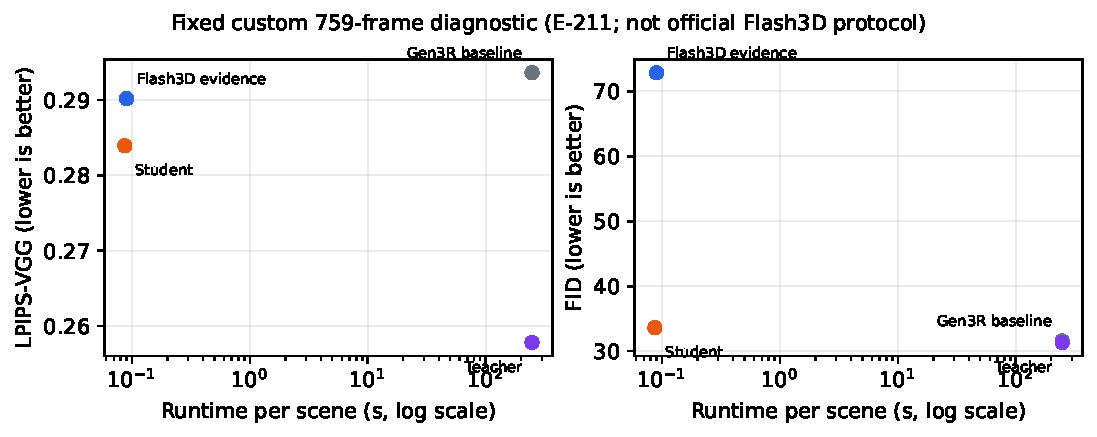
\includegraphics[width=\columnwidth]{fig_quality_speed.pdf}
\caption{Quality--speed vectors from the released E-211 JSON on the same fixed
custom 21-scene/759-frame disocclusion-heavy diagnostic (256$\times$256,
VGG-LPIPS). Flash3D is the geometry/evidence component measured within this
custom diagnostic, not an official-protocol benchmark opponent. Lower is better
on both vertical axes. The student improves over the evidence component at
feed-forward cost but trails the teacher on LPIPS and FID.}
\label{fig:quality-speed}
\end{figure}
\begin{table}[H]
\centering\small
\caption{Exact rounded values behind Fig.~\ref{fig:quality-speed}. These
same-diagnostic measurements support component analysis only; they do not
establish an official-protocol ranking.}
\resizebox{\columnwidth}{!}{%
\begin{tabular}{lrrrr}
\toprule
Method & PSNR$\uparrow$ & LPIPS$\downarrow$ & FID$\downarrow$ & Time \\
\midrule
Gen3R baseline & 17.88 & .294 & 31.6 & 247\,s \\
Flash3D evidence & \textbf{19.98} & .290 & 72.9 & 0.09\,s \\
Teacher (slow) & 19.37 & \textbf{.258} & \textbf{31.3} & 247\,s \\
\textbf{Student (ours)} & 18.17 & .284 & 33.6 & \textbf{0.087\,s} \\
\bottomrule
\end{tabular}%
}
\end{table}
Within this fixed diagnostic, the student records lower LPIPS ($0.284$ versus
$0.290$) and FID ($33.6$ versus $72.9$) than the Flash3D evidence component at
similar measured runtime, but trails the teacher (LPIPS $0.258$, FID $31.3$).
We deliberately restrict this statement to E-211: protocol differences preclude
interpreting it as an official Flash3D result. The released JSON and
\texttt{scripts/generate\_quality\_speed.py} reproduce the quality--speed scatter.

\paragraph{Released checkpoint.}
The package includes the student state dictionary, a model card documenting its
intended use and limitations, and a validation script that verifies the SHA256,
46,371-parameter architecture, state dictionary, and synthetic output shape.

\subsection{Ablation: why not intervene at the Gaussian layer?}
A natural alternative edits the feed-forward backbone's Gaussian attributes
directly. E-150 tests a color-only adapter that changes source-plane
\texttt{features\_dc} and re-renders while freezing means, opacity, scale, and
rotation. It reaches only $\sim$7\% of the teacher$-$baseline gap when overfit on
one scene and does not generalize (holdout $-1.72$ dB). The lower portion of
Fig.~\ref{fig:pipeline} states exactly what this evidence supports: recoloring
existing source-plane Gaussians does not add geometric support where a target
view newly reveals content. The schematic is not a qualitative render result and
does not claim that all Gaussian-space adapters fail; it explains why this tested
color-only, frozen-geometry intervention has limited leverage. We therefore use
an image-space residual over the geometry evidence.

\section{Discussion}
\label{sec:disc}
Within the oracle-selected regime, a tiny feed-forward student retains 94.7\%
(approximately 95\%) of the teacher's disocclusion gain at $\sim$3000$\times$
lower cost with exact visible-region identity. The fixed custom diagnostic
characterizes this quality--speed tradeoff, while the Gaussian-color ablation
explains the chosen intervention level. The result establishes conditional
compressibility of useful teacher behavior, not automatic identification of
where that behavior is useful.

\section{Limitations}
\label{sec:limits}
Final numbers use a high-teacher-gain scene set selected with teacher and
ground-truth outcomes and visibility masks computed from the full target clip.
Both oracle inputs are unavailable for ordinary single-view inference and may
overstate end-to-end performance relative to a practical system. The reported run
used the Flash3D disocclusion basis, offline frame-label weighting, and a
4-scene/161-frame holdout. Released checkpoint evaluation is reproducible, but
exact retraining is partial rather than a self-contained command: external teacher
arrays, the frame-label JSON, and the original holdout manifest are not included,
and the exact scene IDs and frame-label path are unknown in this release. The
released training manifest records the known settings and a placeholder-only
command template. No observable inference-time selector or online visibility
estimator is established. Extending the method beyond the selected regime requires
learning and validating both. An optional stronger adapter could predict residual
disocclusion Gaussians (new points) rather than image-space residuals; this is
separate future work.

\section{Conclusion}
\label{sec:concl}
On an oracle-curated high-teacher-gain regime, the student recovers $+5.77$ dB of
invisible-region PSNR (teacher: $+6.09$ dB; 0.32 dB gap; 94.7\% retained) while
running $\sim$3000$\times$ faster. The visible mask leaves baseline pixels exactly
unchanged inside the evaluated output. The fixed custom 759-frame diagnostic and
Gaussian color-adapter negative ablation delimit what the evidence supports.
Generalization to uncurated scenes remains contingent on future observable
selection and visibility estimation.

{\small
\bibliographystyle{plain}
\bibliography{refs}
}
\end{document}
